%\documentclass[a4paper,12pt]{article}
%\usepackage[english]{babel}
%\usepackage[margin=1in]{geometry}
%\usepackage{setspace}
%\usepackage{graphicx} %for table
%\usepackage[backend=bibtex, style=chicago-authordate]{biblatex}
%\addbibresource{mastersthesis.bib}
%whenever Islandic names
%\usepackage[utf8]{inputenc}
%\usepackage[T1]{fontenc}
\section{Introduction}
The aim of my master's thesis is to (re)construct and study a network of the family ties inside the Swedish Council of the Realm (Riksrådet) from the early 16th century to the late 17th century. The study will be conducted by creating a data structure and a visual representation of a graph depicting the family links. The work will be focused on roughly two main sectors: first of which is the actual analysis of the family links between the councillors, the second one is the assessment of the method of historical network analysis. 

In my thesis historical network analysis will be referred to as a computer-aided method, which links this work to the field of digital humanities. This study is also in the field of pre-modern history, because the timeframe of this study covers most of the 16th and 17th century. Methodologically, the study is quantitative study with an explorative approach.
%TODO political themes

Even though things like machine learning and artificial intelligence (AI) are particularly popular and to a certain degree hyped at the time of writing, it is important to assess and understand the fundamentals and basics of digital and computational methods. Obviously, it is easier to understand simpler models, and therefore ask important questions. Those questions are for instance: What are the premises for this model? What kind of data is suitable for this model? What kind of interpretations can be made from the results? What is the potential problem, how to fix or adjust the model if something goes wrong or unexpectedly?

The text will be divided in four sections. The introduction will present the premises of this work. As the method is a focal point of the study, it will be explained further in its own second section. The third section is about the practical implementation of the analysis and assesment of the results, and the last section collects everything together as a conclusion. 

Furthermore, according to historians Miia Kuha and Petri Karonen, majority of historiography concerning Sweden (and Finland) in the early modern period is written in the national languages Swedish of Finnish.\footcite[p. 6.]{kuha-ja-karonen} 

\subsection{Research questions}
The research questions are:
\begin{enumerate}
	\item Can historical network analysis reveal new or unseen patterns in the affiliations between Swedish councillors of the Realm? \begin{itemize}
		\item How dense is the network (how linked the council was in general)?
		\item Are there any isolated nodes (councillors who have no relatives in the council)?
		\item Can the graph be visually divided into clear subgraphs (is there a certain groups or 'houses' of related councillors)?
	\end{itemize}	
	\item What are the potential difficulties and pitfalls in the implementation and interpretation of historical network analysis in this specific dataset, and further in the field of pre-modern history? \begin{itemize}	
		\item To what extent can pre-processing the dataset for the network analysis be automated with a script?
	\end{itemize}
\end{enumerate} 

The source material for this study is the \textit{Swedish Councillors of the Realm, 1523-1680} dataset, which also dictates the timespan of the study. The period is relatively long and momentous in Swedish history, including many important events, such as, adoption of hereditary kingship (1544), the conflicts between the sons of Gustav Vasa (from 1560's to early 1600's), thirty years war (from 1618 to 1648) and queen Christina abdicating the throne (1654).\footcite[p. 8-9.]{personalAgency} These events and shifts obviously have had a significant impact on the ensemble and activities of the Swedish council of the realm. Yet, instead of event-history or lives of individual councillors, the focus of this study is on the macro level, in (re)constructing a visual and computational network model of the family relations between the councillors. A longer timespan is necessary in order to the generations of family links to accumulate enough to make a network meaningful to study.
%TODO time period after medieval time and before the time of absolutism
%TODO swedish age of greatness (different definitons in pohjoinen suurvalta and sveriges historia)

This study is conducted with a quantitative dataset instead of more traditional way of qualitative text analysis. Therefore, the source criticism is done for the dataset as a whole. For example, by assessing the sources of the dataset, looking for possible human errors in the data and considering the original purpose and use of the dataset. The source criticism is discussed further in the subsection \ref{sources}.

The basis and context of this study will lay on the pre-existing literature concerning the Swedish Council of the Realm. Previous historical research will form the base for deciding the parameters for the network model (graph), and direct the choices for the data processing. These decisions include, for instance, whether or not draw the link between brothers if they are already connected to same father present in the graph. These decisions need to be based on the prior knowledge on the social relations during the pre-modern era. 

\subsection{Previous research}
Historical network analysis can be understood as, to a certain degree established, but developing method. According to Finnish political historians Kimmo Elo and Olli Kleemola, the roots of historical network analysis are as far as in the late 19th century, yet, the modern appliance of the method is due the invention of computers, increase in the computing capacity and availability of user friendly network analysis software. They estimate that historical network analysis has gained its popularity from somewhere in the late 2000's.\footcite[p. 415-417.]{eloAklee15} 

It appears that Elo and Kleemola approach historical network analysis as a predominantly digital or computational research method.\footcite[p. 415-417.]{eloAklee15} However, the definition is not that straightforward. Social network analysis, which is the basis for historical network analysis, involves theorising, model building and empirical research focusing on the patterns formed inside the networks.\footcite[p. 22-24.]{Keats-R2007} (Social) network analysis has been employed in the field of history before the turn of the millenia, previous to the era of intuitive software.\footcite[TODO check!]{AronssonEtA1999} So, the field of historical network analysis can be roughly divided in two approaches: one with more descriptive or theorising stance and the another that treats network analysis as a quantitative computer-aided method. In the context of this work, (historical) network analysis will be treated primarily as a computer-aided method, similarily to the article of Elo and Kleemola, therefore focusing mainly on the previous research with computational approach. The further theory and practice will be covered in the section \ref{method}.

The international \textit{Historical Network Research Community} (HNR) was found in 2009. The community has grown over time, and nowadays HNR runs workshops, conferences, lectures and a Slack (chat) group, and publishes an open access journal, a newsletter and a research bibliography.\footcite{hnr} On the word of Kimmo Elo, historical network analysis has been the most popular computational method amongst historians.\footcite[p. 22.]{elo16} 

Scanning the HNR research bibliography, it appears that historical network analysis has been applied by researchers and research teams from around the globe in variety of research topics. The topics vary from the social networks of Chinese gods to the technical implementation of historical network analysis, and to the historical study of reconnaissance during the Cold War.\footcites[p. 22.]{elo16}{hnrbib} More relevant for this study, network analysis has been utilized in the study of ruling elite and power in the pre-modern period.\footcite[See e. g. Ruth Ahnert's and Sebastian E. Ahnert's book \textit{Tudor Networks of Power} (2023) or Paul D Mclean's article \textit{Widening Access While Tightening Control: Office-Holding, Marriages, and Elite Consolidation in Early Modern Poland} (2004).]{JonVidarEt} 
 
In Finland, Kimmo Elo is one of the researchers highly profiled on the use of the historical network analysis. Among other things, he has co-authored two articles addressing the method in more explorative manner. The first article is "\textit{Verkostoanalyysi historiallisten aineistojen eksploratiivisena analyysimenetelmänä : esimerkkinä sotavalokuvat}" written by Elo and Olli Kleemola. In the article they focus mainly on the applicability of historical network analysis. As their data, they use German war propaganda pictures taken from Finland during the second world war.\footcite{eloAklee15}

The another article is "\textit{Networks of Revolutionary Workers: Socialist Red Women in Finland in 1918}" written by Elo and political historian Tiina Lintunen. In this article the method of historical network analysis is applied on the connections between the women who participated to the Finnish civil war in 1918 on the side of the socialists also known as "reds".\footcite[Almost the same article is found in Finnish in the \textit{Historiallinen Aikakauskirja} 116 (2/2018).]{LintunenAndElo2019} Both of these articles share the exploratory perspective with this study, and therefore, offer a point of reference. 

When it comes to the literature discussing early modern Sweden, historian Petteri Impola has made a quantitative analysis on the social groups studied by Swedish and Finnish historians. Generally the early modern royals and nobility was the the focal point within the Swedish scholars till the 1950's, whereas their Finnish colleques have been more focused on the peasants and other proletarian groups. Overall, in the latter half of 20th century more attention was paid towards lower social classes. Yet, a resurgence of interest in the nobility has occured in the beginning of the 21st century. This new research examining nobility has been focusing on women, family connections and further social networks.\footcite{impola2024} My work seems to be similar with the modern study of the nobility.

As a significant administration the members and activities of the Swedish Council of the Realm have been to some extent covered by previous research. For instance, the development and affairs of the council as an institution are addressed in the works of historians such as Petri Karonen, Pentti Renvall and Kurt Agren.\footnote{See e. g. Petri Karonen: \textit{Pohjoinen Suurvalta} (2008) TODO check! or "\textit{The council of the realm and the quest for peace in Sweden, 1718-1721}" in \textit{Hopes and fears for the future in early modern Sweden, 1500-1850} (2009), Pentti Renvall "\textit{Keskitetyn hallintolaitoksen kehitys}" in \textit{Suomen kulttuurihistoria. II} (1934) or Kurt Agren "\textit{Rise and decline of an aristocracy: The Swedish social and political elite in the 17th century}" in the \textit{Scandinavian journal of history} (1976).} Additionally, short biographies of some members of the council can be found easily in the \textit{Biografiskt lexikon för Finland} (Biographical Dictionary of Finland).\footcite{blf} Those biographies include an assortment of notables found in the councillors dataset, such as, Herman (Claesson) Fleming, Gabriel Bengtsson Oxenstierna (af Korsholm och Wasa) or Lorentz (Ernstsson) Creutz d.ä.\footcite{blf-list} Even so, the Council of the Realm has not been examined thoroughly down to the last man. And based on historians Marko Hakanen and Ulla Koskinen, the council as a focal point, does still hold some uncovered parts.\footcite[p. 47-48.]{HakanenAKoskinen2017} 

Authors of the councillors dataset, Hakanen and Koskinen, have explained the dataset's background in their article \textit{The Gentle Art of Counseling Monarchs (1560-1655)}. In their study the council is approached through the concept of personal agency.\footcite{HakanenAKoskinen2017} In the article, Hakanen and Koskinen also mention some prior collection and utilisation of datasets on the study of said councillors and their networks. Namely, Jan Samuleson has listed councillors and their affiliations from years 1523 – 1611, Kurt Ågren has collected councillors and their families from years 1602 – 1647, and Björn Asker made a similar collection from years 1640 – 1680. Unfortunately, some of the datasets remain unpublished.\footcite[p. 48, 67 (cite 4).]{HakanenAKoskinen2017} 

All in all, computer-aided historical network analysis is somewhat rare compared to the traditional methods of historiography. Nevertheless, it also seems that the pre-modern elite is collectively understood as a network amongst historians, and the ties between the members of nobility have been in the scope of interest for some time now. Which makes applying the computer-aided network analysis relevant. The aim of this work is to join the rather uncommon method of historical network analysis with the classic research topic, and to further explore and develop the method in the context of historical research.

\subsection{The Council of the Realm}
\begin{quote}
	The position of the councillors of the realm was well recognized by the whole society. They were an elite group which enjoyed formal position in the power structure. Their job was to help the monarch reach decisions.\footcite[p. 26.]{agencyAndStateBuilding}
\end{quote}

In the early modern Sweden the Council of the Realm (Privy Council, swe. Riksrådet, fi. valtaneuvosto) was to give council to the Royal Majesty (monarch, king or queen) on decision making. The Council consisted of noblemen loyal to the monarch. The councillors held a signifficant power and authority on the realm, yet, the Council did not have the ability to make decisions bypassing or opposing the monarch. Ideally decisions would be made in concensus with the king or queen and the Council.\footcites[p. 13-14,]{hopesAndFearsIntro}[p. 47-50.]{HakanenAKoskinen2017}

The position of the Council as an institution was established in the early Middle Ages. With the elective kingship in the medieval period, the elections of Swedish kings were made with the consent of the Council. The authority and power possessed by the Council fluctuated from time to time, but it is said to been been on in its peak during the 15th century. However, in the early decades of the 16th century, the Council took part in the plot against the personal union of Sweden and Denmark \textit{Kalmar Union} (1397-1523) and the Danish king. Consequently, ten councillors lost their lives in the dramatic events of \textit{Stockholm Bloodpath} or "the coronation of King Christian II of Denmark" in November 1520. These occurrences soon lead to the splitting of the Kalmar Union and Gustavus Vasa's (1495/1496-1560) rise to power.\footcites[p. 49-50,]{HakanenAKoskinen2017}[p. 8-9.]{personalAgency}

Following Gustavus Vasa's and his descendants accessement of the throne, the authority and power of the Council and upper aristocracy weakened. The Council was only called on by the king, further, the king was the one who chose the members of the Council, hence being able to favour the ones conforming him.\footcite[p. 58.]{pSuurvalta} Gustavus Vasa and his sons percieved the upper aristocrats as rivals, therefore relying on the unoffical help and support of their ignoble\footnote{Nonaristocratic, proletarian.} secretaries.\footcite[p. 53.]{HakanenAKoskinen2017}

Overall, the timeperiod between 1560 and 1611 was politically turbulent and unpredictable in the Swedish realm. The passing of Gustavus Vasa in 1560 lead to the bitter rivalry and struggle over the inheritance of the throne between his three sons. Each of his sons ruled Sweden for relatively short period of time, and the unforeseen changes of monarchs meant that the Council and nobility had to adapt and swear allegiance to the right sovereign at the right time. Loyalty to the wrong party lead to fall from favour at best or execution at worst. It can be considered essentially dangerous to be in a position of power during that timeperiod.\footcites[p. 96-121,]{pSuurvalta}[p. 51-52.]{HakanenAKoskinen2017}

The Council faced the the most severe crisis during the 1590's civil war. The warfare over Swedish throne was fought between Gustavus Vasa's youngest son Duke Charles (future king Charles IX 1550-1611) and Gustavus Vasa's grandson the king of Poland Sigismund. The war lead to the Duke Charles' rise to power, and the demise of the noblemen and councillors who had opposed him.\footcites[p. 57-60,]{HakanenAKoskinen2017}[p. 96-121.]{pSuurvalta} In fact, the Council was practically decimated in 1601, nonetheless, the kingdom needed the help of a legitime Council in order to take care of the administrative and diplomatic tasks. In 1602 Duke Charles appointed 15 new councillors.\footcite[p. 57-59.]{HakanenAKoskinen2017}

After the death of Charles IX in 1611, Charles' oldest son Gustavus Adolphus (Gustav II Adolf 1594-1632) became the king. At that time, the kingdom was at war with Denmark. To appease the nobility and settle the political situation within Sweden, Gustavus Adolphus gave a charter of guarantees, which, for example assured all of the high posts in civil administration to the nobility by privileges.\footcites[p. 121-123,]{pSuurvalta}[p. 8-9.]{personalAgency} The authority and position of the aristocracy and the Council incremented significantly in the early 17th century. Due that, the Council was able to set the Regency (swe. Förmyndarregering, fi. holhoojahallitus) after the king's sudden death in 1632. Additionally, the Council started to gather recurringly in Stocholm. The 1634 Instrument of Government (swe. regeringsform, fi. valtiomuoto) further warranted the position of the nobility and the Council.\footcites[p. 195-197,]{pSuurvalta}[p. 16-17,]{agencyAndStateBuilding}[p. 8-9.]{personalAgency}

The position of the nobility and the Council started to decline drastically after the Charles XI's (1655-1697) succession of the throne in 1672. In the Diet of 1680 the monarch practically retracted the status of the Council. In 1681 the Council of the Realm was renamed the \textit{Royal Council} (swe. Kungligt råd, fi. kuninkaallinen neuvos). Concurrently, the Great Reduction was being implemented, meaning that the fiefs\footnote{Lands given to the aristocracy.} were reclaimed to the state. The reign of Charles XI is retroactively called the Age of Absolutims in Sweden.\footcites[p. 289-295,]{pSuurvalta}[p. 8-9.]{personalAgency} Finally, in the 18th century the role of the Council steadily declined further, and it was disestablished during the reign of Gustavus III (1772-1792).\footcite[p. 14.]{hopesAndFearsIntro}

\begin{table}
	\caption{Parameters on the number of councillors between 1520-1680.(\cite{councillorsDS}) Calclutaed with R script: https://github.com/Heidi-Suurkaulio/mastersthesis/tree/main/RScripts}
	\label{tab:councillors}
	\centering
\begin{tabular}{c c c c c c}
	\hline
	Min. & 1st Qu. & Median & Mean & 3rd Qu. & Max.\\
	\hline
	1.00 & 19.00 & 23.00 & 24.29 & 27.00 & 48.00\\
	\hline
\end{tabular}
\end{table}

\begin{figure}[h]
	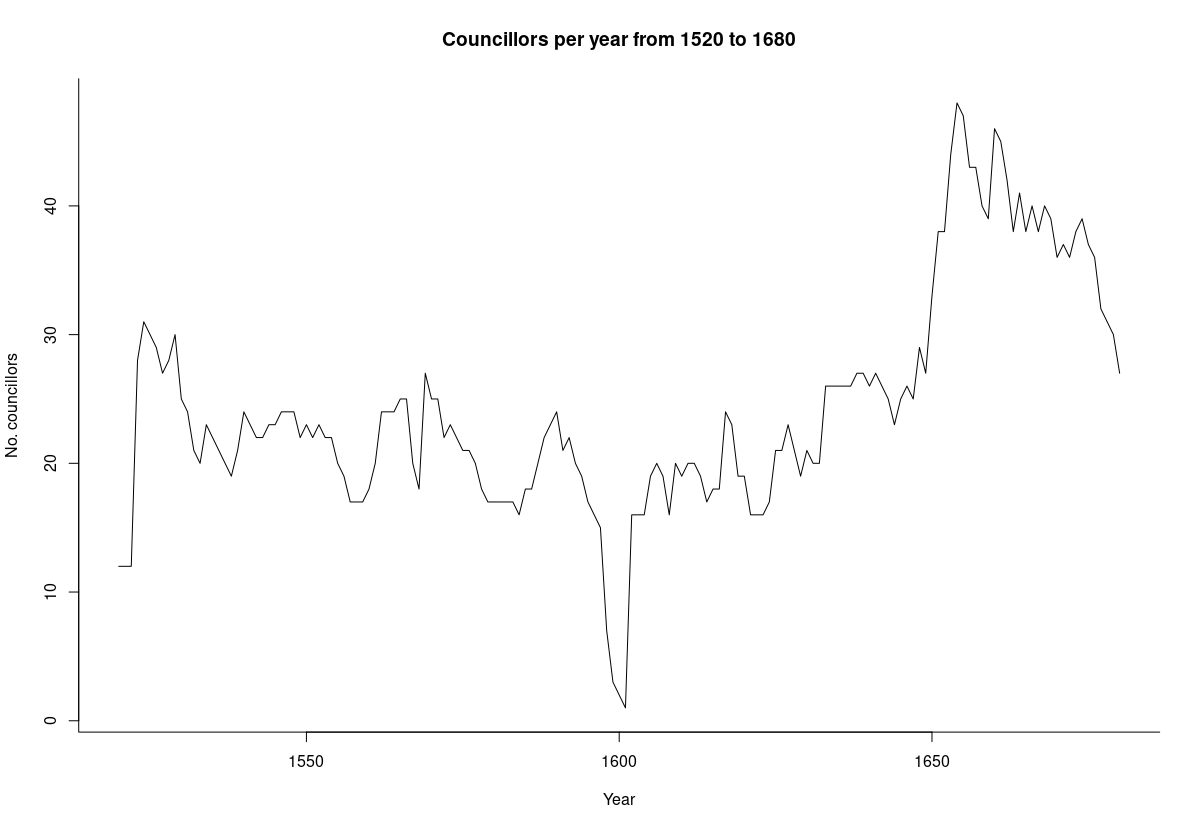
\includegraphics[width=\linewidth]{councillorsPerYear.png}
	\centering
	\caption{The changes of the number of councillors per each year.(\cite{councillorsDS}) Plotted with R script: https://github.com/Heidi-Suurkaulio/mastersthesis/tree/main/RScripts} 
	\centering
	\label{fig:peryear}
\end{figure}

The 1442 Law of Realm ordered the Council to be consisted of 12 noble men and varying number of bishops and other clerics.\footcite[p. 49.]{HakanenAKoskinen2017} As the religious reformation was implemented during the reign of Gustavus Vasa, the bishops and church men lost their position in the Council. Thereafter, the Council consisted primarily of noble men during the 1523-1680 time period.\footcites[p. 72-75,]{pSuurvalta}[p. 15]{agencyAndStateBuilding} 

According to the \textit{Swedish councillors of the Realm, 1523-1680} -dataset, between 1520 and 1680 the number of active councillors per year changed between 1 in 1601 to 48 in 1654, the mean being 24.29 and median 23. Most of the time the number was between 19 and 27 (Table \ref{tab:councillors}).\footnote{Median is the middle observation on the data, it usually represents the middle point of the distribution.\cites[p. 26,]{statisticsfor}[p. 30-31.]{MooreEtAl} 1/2 (50\%) of the observations lay between the 1st and 3rd quartile.\cite[p. 32-33.]{MooreEtAl}} The fluctuation of the councillors count is visible in the Figure \ref{fig:peryear}. 

Generally, it seems that the broader position of the Council and the enclosing aristocracy is proportional to the amount of the councillors. However, such an abstract and broad concept as 'position' should be understood as a \textit{latent variable}. Latent variable meaning a factor that is mesurable and observable only indirectly through modeling and calculating other variables.\footcite{apa}. As well as the definition of 'position' as a concept not being that simple and straight forward. It cannot be indubitably quantified in one diagram.

In Figure \ref{fig:peryear}, the amount of councillors declined during the religious reformation in the first half of the 16th century. Then the political instability is seen in the downward spikes after year 1560, most dramatic of those being in the turn of the 16th and 17th century. The amount started a rapid incline somewhere mid 17th century and hit its peak in 1654. It being the year queen Christina (1626-1689) relinquished the throne to her cousin Charles X Gustav (1622-1660).\footcite[p. 8-9.]{personalAgency} According to Hakanen and Koskinen queen Christina could also have deliberately raised the number of councillors in order to dilute their power.\footcite[p. 63-64.]{HakanenAKoskinen2017} Yet, closing the year 1680 the number starts to drop exceedingly.

In early modern Sweden the monarch was the highest authority. Practically the deeds of the royal family members were on the second place, and the power of the Council came afther these two. Beneath these was the Diet of Sweden (swe. Riksdag, fi. valtiopäivät): the representatives of the four estates–the Nobles, the Clergy, the Burghers and the Peasants–that was to negotiate and legitimate the rules and laws given by the monarch.\footcite[p. 57-61.]{pSuurvalta}  All in all, the place in the Council of the Realm was highly sought after, and compared to the surrounding society or even encompassing nobility, the members enjoyed a significant valuation, authority and most of the time prosperity and wealth.

\subsection{Sources}
\label{sources}
Since this work is conducted with pre-collected dataset, this work can be vaguely categorized as secondary analysis. Secondary analysis meaning re-analyzing the data with new research questions or approaches, while primary analysis involves the collection of the data. Secondary analysis can also be discerned from meta analysis, which means comparing multiple previous studies (usually with quantitative methods) to create a synthesis on a certain question.\footcite[p. 4-5.]{meta-analysis} 

On the contrary in their articles Kimmo Elo and Olli Kleemola or Elo and Tiina Lintunen apply a network analysis on their own primary datasets.\footcites{eloAklee15}{LintunenAndElo2019} However, in the case of this work the benefit of doing secondary analysis is that the focus can be on the implementation and assessment of the method. Furthermore, the existing dataset will be automatically and manually re-examined for possible errors in the process, as will be discussed soon. 

As mentioned earlier, this work is based on the \textit{Swedish councillors of the Realm, 1523-1680} -dataset authored by Marko Hakanen and Ulla Koskinen. The dataset was published in 2017 and can be found in Digital repository of University of Jyväskylä under the license CC BY 4.0. The dataset was collected as a part of the research conducted for the anthology \textit{Personal Agency at the Swedish Age of Greatness 1560–1720}.

To be precise, discussing the data I deliberately use the term \textit{dataset}, whereas the original authors call it \textit{database}. The difference between dataset and database is not clear-cut, but for example the U.S. Geological Survey (USGS) compactly defines dataset as a structured collection of data and database as a collection of multiple datasets. USGS also mentions that the data in databases can (typically) be updated and manipulated easily in real time.\footcite{usgs} Hence, databases are generally more complicated interfaces for data management, and for this purpose the term dataset is more suitable.

The dataset consists of information from 257 Swedish councillors of the realm. Each councillor has the following feature attributes: date of birth, year of death, year, date and age of appointment, noble rank, spouse(s) along with father's spouse and the individual's family links between other councillors. The councillors are identified with their full name and id number.\footcites[p. 48.]{HakanenAKoskinen2017}{councillorsDS}
%table was here

Hakanen and Koskinen have compiled the data from secondary sources such as biographical registers and databases, biography collections, lineage databases and research literature. The dataset's sources are listed in the dataset and in the article written by Hakanen and Koskinen, those include for instance Nordic Family Book (Nordisk familjebok), National Biography of Finland (Finland's nationalbiografi, Kansallisbiografia), genealogies of old Swedish aristocratic families (Äldre svenska frälsesläkter) and further refereed literature.\footcites[p. 48, 76]{HakanenAKoskinen2017}{councillorsDS} As reported by Hakanen and Koskinen the dataset is collected using methodologies of collective biography, new prosopography and source criticism.\footcite[p. 48.]{HakanenAKoskinen2017}
  
Even though the dataset can be assessed as reliable and generally accurate, there is the general problem of some missing data. As seen in the example of Table \ref{tab1}, some of the councillors have missing attributes such as date of birth and therefore age of appointment. The missing attributes are most likely due the fact that during the time span of the dataset there was no standard of civil registration. 

The order of keeping parish registers (kyrkbok) was given in the Swedish Church Law 1686 (Kyrkio-Lag och Ordning), six years from the endpoint of the dataset. The Church Law made it mandatory for parish vicars to keep certain records and documents concerning the population and economy of the parish. Among other things these parish registers included the records of marriages, births, christens, deaths and funerals. Despite that the Swedish parish registers have been assessed exceptionally comprehensive by historians, there are some considerable deficiencies due to the differing circumstances and practices between parishes, furthermore some of the registers have been destroyed or lost. Even though some records do exist prior and post (TODO format) the Swedish Church Law 1686, they are notably dispersed.\footcite[p. 169-176.]{viikki94} A case in point: according to the Dictionary of Swedish National Biography (Svenskt biografiskt lexikon) the birth year of king Gustav Vasa (1495 or 1496) is also an estimate.\footcite{sbl_gustav_v} 

However, the focus of this work is not on the ages of the councillors but in their affiliations, so, the more relevant question is whether or not there are missing family links. 

(TODO write script and do some checking)

As the relatively large dataset is compiled by humans, it leaves some room for typos and errors. While producing the first experimental graph of the dataset, some empty data points were found. These "ghosts" were nodes with only id number and one or two links to the other councillors. All in all there were four "ghosts" with the id numbers 147 (linked to 18 and 152), 215 (linked to 217), 249 (linked to 269) and 254 (linked to 94). With the help of Marko Hakanen it was resolved that those "ghost" nodes were data points removed from the dataset as the authors found out they have not been official councillors, however, some references to their id numbers had been left to the dataset by accident. The "ghost" nodes will be removed from the latter graphs.

% TODO excluding women and lower classes

\begin{sidewaystable}
	\caption{Example rows of the dataset: Gyllenhorn, Joen Olsson and Natt och Dag, Måns Johansson (\cite{councillorsDS})}
	\label{tab1}
\resizebox{\textwidth}{!}{%
	\begin{tabular}{|c | c | c | c | c | c | c | c | c | c|}
		\hline
		Name & No. & D.O.B. & † & Appointed & Date & Age & Noble rank & Family members in the council & Spouse(s) / Father of Spouse / Date of Marriage \\ 
		\hline
		Gyllenhorn, Joen Olsson & 82 & & 1556 & 1529 & 00.6. & & Uradel (Ancient Nobility) & Son-in-law 44 & Karin Bese/Nils Nilsson Bese/1529 \\
		\hline
		Natt och Dag, Måns Johansson & 142 & 1498 & 1555 & 1529 & 00.6. & 31 & Uradel (Ancient Nobility) & & Barbro Eriksdotter/Erik Turesson Bielke/ probably 27.6.1524 \\
		\hline
	\end{tabular}%
}
\bigskip
	\caption{Example of the raw .csv file}
	\resizebox{\textwidth}{!}{%
		\begin{tabular}{|cccccccccp{1.5in}p{1.5in}|}
			\hline
			1 &Name; &Id; &D.O.B.; &died; &Appointed; &Date; &Age; &Noble rank; &Family; &Spouse(s) / Father of Spouse / Date of Marriage \\
			\hline
			2 &Ingemar Petri; &162; &; &1530; &1495; &; &; &Estate unknown, Bishop; &; &; \\
			\hline
			3 &Tre Rosor, Ture Jönsson; &231; &; &1532; &1497; &; &; &Uradel (Ancient Nobility); &Father CR, Father-in-law CR, Sons 228, 230, Son (illegitimate) 175; &Anna Johansdotter/ Johan Christiernsson Vasa (CR) \\
			\hline
		\end{tabular}%
	}
\end{sidewaystable}